\documentclass[11pt,a4paper]{article}
\usepackage[utf8]{inputenc}
\usepackage[T1]{fontenc}
\usepackage[brazil]{babel}
\usepackage{amsmath}
\usepackage{amssymb}
\usepackage{booktabs}
\usepackage{graphicx}
\usepackage{subcaption}
\usepackage{xcolor}
\usepackage{geometry}
\geometry{margin=2.5cm}

\title{\textbf{Mundo de Wumpus com SARSA}\\[0.4em]
\large Aula 18 --- Aprendizado por Refor\c{c}o}
\author{Breno Porto Pinheiro do Prado \quad RA 185196 \\ Guilherme Bento Ramos \quad RA 185226}
\date{}

\begin{document}
\maketitle

\section{O Exerc\'icio}

O objetivo \'e aplicar o algoritmo \textbf{SARSA} ao Mundo de Wumpus cl\'assico, partindo da
implementa\c{c}\~ao anterior em Rust (agente BFS baseado em modelo). O trabalho cobre
tr\^es fases: \textit{(i)} treinar o agente num mapa fixo; \textit{(ii)} testar o modelo treinado num mapa
diferente sem re-treinamento (zero-shot); \textit{(iii)} adaptar o modelo ao novo mapa via fine-tuning.

\subsection{Ambiente}

Grade $4\times4$: P=abismo, W=Wumpus, G=ouro. O agente come\c{c}a em $(0,0)$ voltado para
a direita e disp\~oe de uma flecha. Ele percebe \textit{brisa} (pit adjacente), \textit{cheiro} (Wumpus
adjacente) e \textit{brilho} (ouro na casa atual), mas n\~ao v\^e o mapa diretamente. A miss\~ao \'e
pegar o ouro e retornar \`a entrada.

\paragraph{Mapas}

Os dois mapas foram projetados para testar um aspecto espec\'ifico de generaliza\c{c}\~ao: no
mapa de treino o ouro est\'a no extremo \textbf{direito} da linha base; no de teste est\'a no extremo
\textbf{superior esquerdo}. O agente treinado a se mover para a direita tem que reaprender a
dire\c{c}\~ao de explora\c{c}\~ao --- um teste de transfer\^encia negativa deliberado.

\begin{figure}[h]
\centering
\begin{subfigure}[b]{0.3\textwidth}
\centering
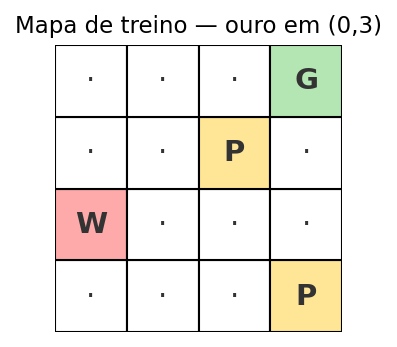
\includegraphics[width=\textwidth]{figuras/grid_train.png}
\caption{Mapa de treino --- ouro em $(0,3)$}
\end{subfigure}
\hspace{3cm}
\begin{subfigure}[b]{0.3\textwidth}
\centering
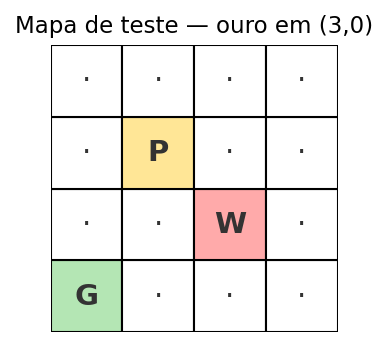
\includegraphics[width=\textwidth]{figuras/grid_test.png}
\caption{Mapa de teste --- ouro em $(3,0)$}
\end{subfigure}
\caption{A=in\'icio, G=ouro, P=abismo, W=Wumpus. Linha~0 \'e a base.}
\end{figure}

\section{SARSA e Configura\c{c}\~ao}

\subsection{Algoritmo}

SARSA \'e controle TD on-policy: a atualiza\c{c}\~ao usa a a\c{c}\~ao que \textit{ser\'a de fato tomada} no
pr\'oximo passo ($a'$), n\~ao o m\'aximo sobre todas as a\c{c}\~oes como no Q-Learning.
\begin{equation}
Q(s, a) \leftarrow Q(s, a) + \alpha\bigl[r + \gamma\,Q(s', a') - Q(s, a)\bigr]
\end{equation}
Isso torna o agente mais conservador: aprende a considerar o risco de explora\c{c}\~ao
($\epsilon$-greedy) como parte da pol\'itica, evitando beiras de abismos durante o treino.

\subsection{Representa\c{c}\~ao de estado}
\begin{equation}
s = (r,\,c,\,d,\,g,\,f,\,w,\,\textit{brisa},\,\textit{cheiro},\,\textit{brilho})
\;\in\; \mathbb{Z}_4^2 \times \mathbb{Z}_4 \times \{0,1\}^6
\end{equation}
O espa\c{c}o tem $4\times4\times4\times2^6 = 4096$ estados e $4096\times6 = 24\,576$ pares (estado, a\c{c}\~ao).
A tabela Q \'e um dicion\'ario Python com valor padr\~ao 0; somente os estados visitados
ocupam mem\'oria.

\subsection{Recompensas}

\begin{table}[h]
\centering
\begin{tabular}{lc}
\toprule
Evento & Recompensa total \\
\midrule
Passo normal (girar) & $-1$ \\
Bater na parede      & $-2$ \\
Morte (abismo/Wumpus) & $-1001$ \\
Flecha acerta Wumpus & $+49$ \\
Pegar ouro           & $+99$ \\
Sair com ouro        & $+999$ \\
Sair sem ouro        & $-51$ \\
Subir fora da entrada & $-11$ \\
\bottomrule
\end{tabular}
\end{table}

\subsection{Hiperpar\^ametros}

\begin{table}[h]
\centering
\begin{tabular}{lll}
\toprule
Par\^ametro & Valor & Nota \\
\midrule
$\alpha$ & 0,10 & Aprendizado est\'avel sem oscilar \\
$\gamma$ & 0,95 & Valoriza recompensas futuras \\
$\epsilon_0$ / $\epsilon_{\min}$ & 1,0 / 0,02 & Explora\c{c}\~ao total $\to$ residual \\
Decaimento de $\epsilon$ & 0,9995 & Chega ao m\'inimo em $\approx$8\,000~ep. \\
Epis\'odios (treino) & 10\,000 & \\
Epis\'odios (fine-tuning) & 5\,000 & Mapa novo \'e mais dif\'icil \\
$\epsilon$ no fine-tuning & 0,50 & Explora\c{c}\~ao alta para sair do h\'abito anterior \\
\bottomrule
\end{tabular}
\end{table}

\section{Resultados}

\subsection{Treinamento --- mapa fixo}

\begin{figure}[h]
\centering
\begin{subfigure}[b]{0.48\textwidth}
  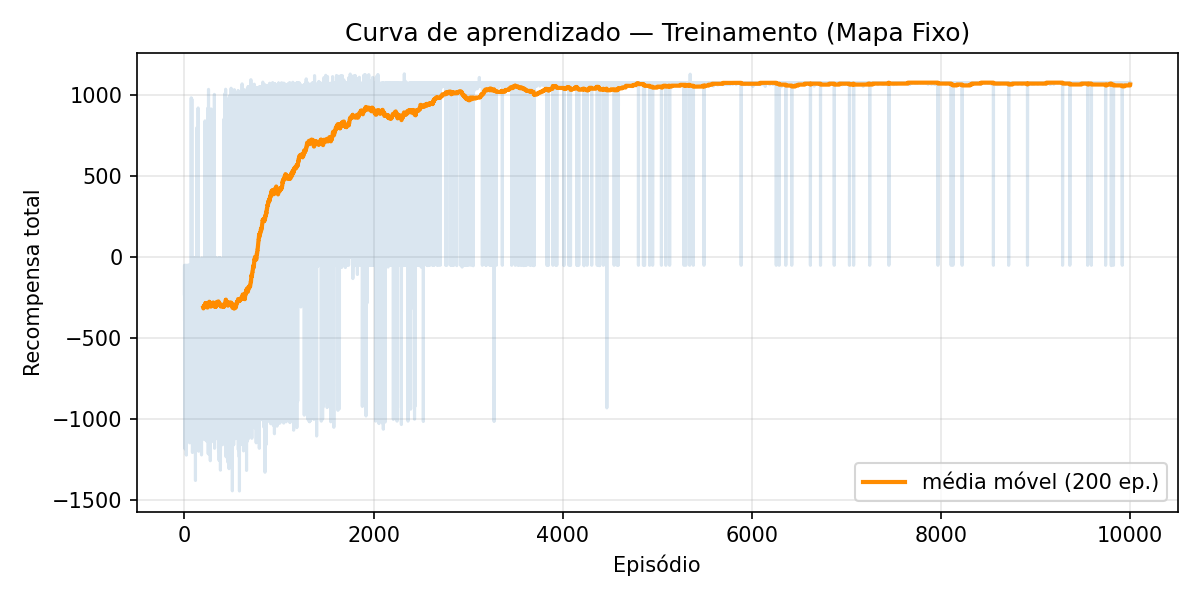
\includegraphics[width=\textwidth]{figuras/sarsa_train_rewards.png}
  \caption{Recompensa por epis\'odio}
\end{subfigure}
\hfill
\begin{subfigure}[b]{0.48\textwidth}
  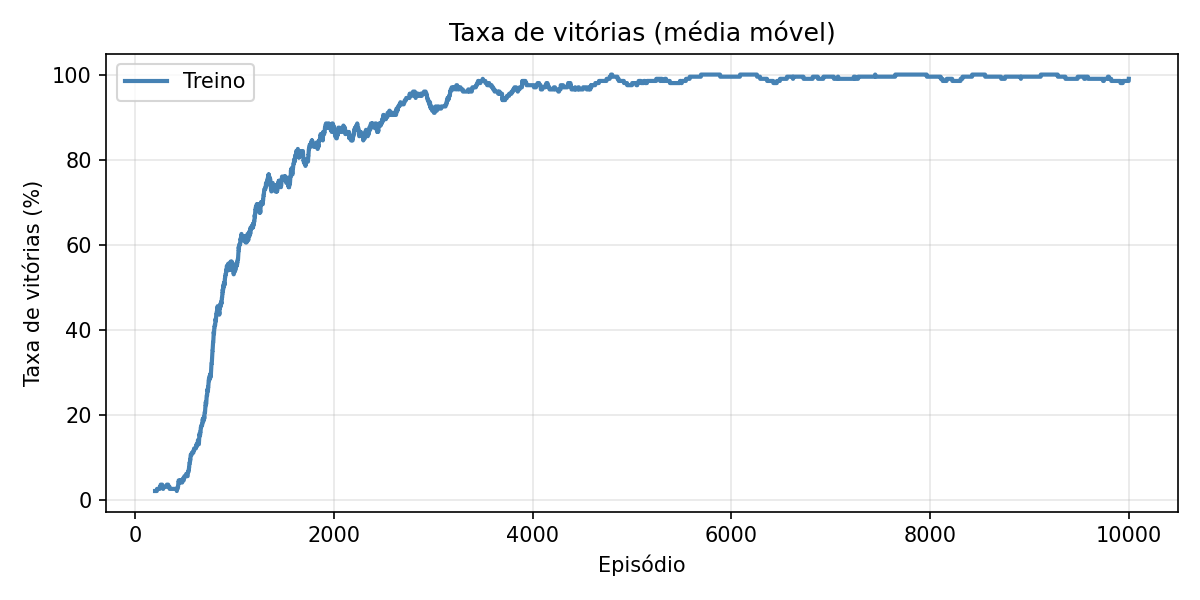
\includegraphics[width=\textwidth]{figuras/sarsa_win_rate_train.png}
  \caption{Taxa de vit\'orias}
\end{subfigure}
\caption{Curvas de aprendizado no mapa de treino (10\,000 epis\'odios).}
\end{figure}

\begin{table}[h]
\centering
\caption{Avalia\c{c}\~ao no mapa de treino (200 epis\'odios, $\epsilon=0$).}
\begin{tabular}{lr}
\toprule
Vit\'orias & 200/200 (100\%) \\
Mortes     & 0/200 (0\%) \\
Recompensa m\'edia & 1079 \\
Passos m\'edios    & 11 \\
\bottomrule
\end{tabular}
\end{table}

O agente converge para uma pol\'itica perfeita. A solu\c{c}\~ao encontrada (11 passos): avan\c{c}a
pela linha 0 at\'e o ouro em $(0,3)$ atravessando $(0,2)$ com brisa, pega o ouro, gira e retorna.
Um tiro \'e disparado desnecessariamente em $(0,1)$ --- comportamento sub\'otimo herdado
de estados em que matar o Wumpus era valioso e que compartilham a mesma entrada na
tabela~Q.

\subsection{Transfer\^encia zero-shot --- mapa de teste}

\begin{table}[h]
\centering
\caption{Avalia\c{c}\~ao no mapa de teste sem re-treinamento.}
\begin{tabular}{lr}
\toprule
Vit\'orias & 0/200 (0\%) \\
Mortes     & 181/200 (90,5\%) \\
Timeouts   & 19/200 (9,5\%) \\
Recompensa m\'edia & $-1086$ \\
Passos m\'edios    & 62 \\
\bottomrule
\end{tabular}
\end{table}

Zero vit\'orias. O agente vai direto para a direita (como aprendeu no treino), mas no
novo mapa o ouro est\'a em $(3,0)$ --- exige ir para \textbf{cima}, n\~ao para a direita. Ap\'os entrar
em $(0,1)$ e sentir brisa, fica preso tentando a\c{c}\~oes do repert\'orio treinado (\texttt{climb} fora da
entrada, \texttt{grab} sem ouro, \texttt{shoot} sem alvo) at\'e eventualmente cair no abismo em $(1,1)$. Este
\'e um caso claro de \textbf{transfer\^encia negativa}: o conhecimento adquirido n\~ao apenas n\~ao
ajuda --- ele atrapalha ativamente.

\subsection{Fine-tuning --- mapa de teste}

\begin{figure}[h]
\centering
\begin{subfigure}[b]{0.48\textwidth}
  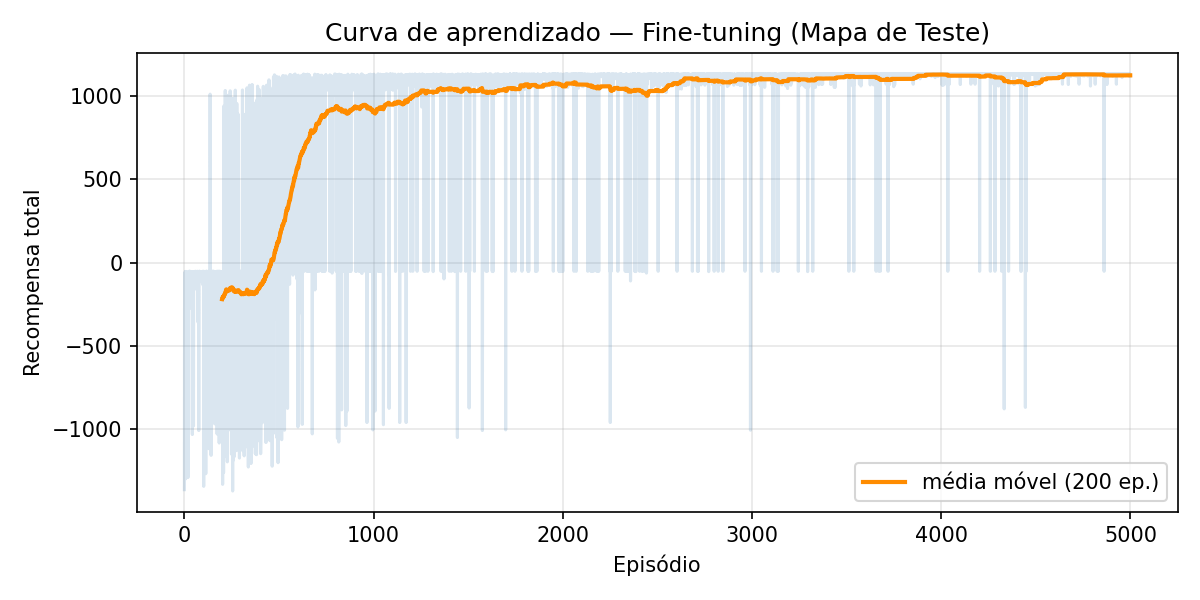
\includegraphics[width=\textwidth]{figuras/sarsa_ft_rewards.png}
  \caption{Recompensa por epis\'odio}
\end{subfigure}
\hfill
\begin{subfigure}[b]{0.48\textwidth}
  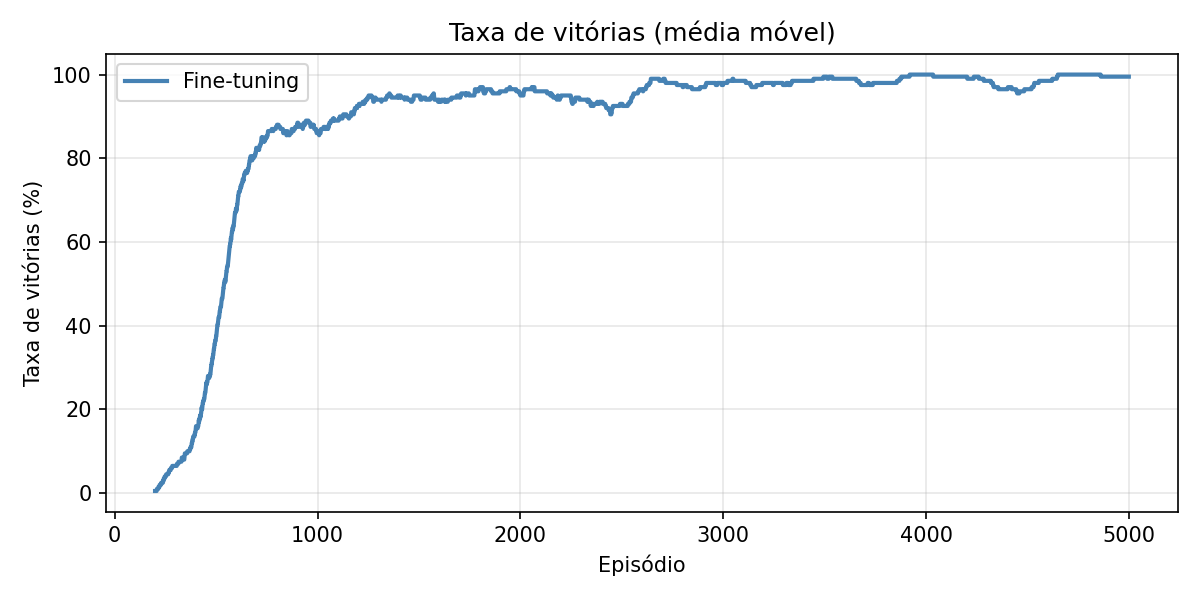
\includegraphics[width=\textwidth]{figuras/sarsa_win_rate_ft.png}
  \caption{Taxa de vit\'orias}
\end{subfigure}
\caption{Fine-tuning no mapa de teste (5\,000 epis\'odios, $\epsilon_0 = 0.5$).}
\end{figure}

\begin{table}[h]
\centering
\caption{Avalia\c{c}\~ao no mapa de teste ap\'os fine-tuning.}
\begin{tabular}{lr}
\toprule
Vit\'orias & 200/200 (100\%) \\
Mortes     & 0/200 (0\%) \\
Recompensa m\'edia & 1134 \\
Passos m\'edios    & 16 \\
\bottomrule
\end{tabular}
\end{table}

Com 5\,000 epis\'odios adicionais e $\epsilon$ reiniciado em $0{,}5$, o agente atinge 100\% de vit\'orias.
A solu\c{c}\~ao aprendida (16 passos) mata o Wumpus em $(2,2)$ com tiro pelo corredor da
coluna~2, navega at\'e $(3,0)$ ao longo da linha~3 e retorna pela coluna~0. Essa rota \'e mais
longa que o \'otimo te\'orico (11 passos pela coluna~0), mas evita a brisa sentida em $(1,0)$
--- o agente preferiu o caminho que parecia mais seguro durante a explora\c{c}\~ao.

\begin{table}[h]
\centering
\begin{tabular}{lcccc}
\toprule
Fase & Vit\'orias & Mortes & Recomp.\ m\'edia & Passos m\'edios \\
\midrule
Treino p\'os-treinamento  & 100\% & 0\%   & 1079   & 11 \\
Teste zero-shot           & 0\%   & 90,5\% & $-1086$ & 62 \\
Teste p\'os fine-tuning   & 100\% & 0\%   & 1134   & 16 \\
\bottomrule
\end{tabular}
\end{table}

\section{An\'alise}

\subsection{Transfer\^encia negativa}

A queda de 100\% para 0\% entre treino e zero-shot n\~ao \'e falha do algoritmo: \'e consequ\^encia
de uma mudan\c{c}a \textit{estrutural} no layout do mapa. O estado $(0,0,\to,\text{sem percep\c{c}\~oes})$ tem
Q-values altos para \texttt{forward} ($\to$ direita) porque essa a\c{c}\~ao levava ao ouro no treino. No
mapa de teste, o mesmo estado existe mas \texttt{forward} leva para longe do ouro.

Os \'unicos comportamentos que genuinamente generalizam s\~ao os \textbf{perceptuais}: \texttt{grab}
quando $\textit{brilho}=1$ e \texttt{climb} quando em $(0,0)$ com ouro. Esses nunca s\~ao ativados no zero-shot porque o agente nunca chega ao ouro.

\subsection{SARSA vs.\ Q-Learning neste dom\'inio}

A caracter\'istica on-policy do SARSA \'e uma vantagem pr\'atica aqui: durante o treino,
quando a pol\'itica $\epsilon$-greedy explora perto de abismos, o SARSA penaliza esses estados
considerando que a pr\'oxima a\c{c}\~ao pode ser aleat\'oria e perigosa. O resultado \'e uma pol\'itica
mais cautelosa em rela\c{c}\~ao a brisas e cheiros, o que explica a prefer\^encia pelo caminho mais
longo (mas percebido como mais seguro) no mapa de teste.

\subsection{Custo do fine-tuning}

O fine-tuning custou 5\,000 epis\'odios para um mapa com solu\c{c}\~ao de 16 passos. A dificuldade principal foi desfazer o h\'abito de ir para a direita: nos primeiros 500 epis\'odios
as primeiras vit\'orias mal aparecem. A partir do epis\'odio 1000 a converg\^encia \'e r\'apida,
indicando que o conhecimento residual (como retornar a $(0,0)$ depois de pegar o ouro) foi
reutilizado e acelerou o aprendizado da nova rota.

\subsection{Limita\c{c}\~oes}

\begin{itemize}
  \item A tabela Q cresce com $O(N^2)$ em grades maiores; DQN seria necess\'ario.
  \item O reward shaping (b\^onus por ouro e kill) \'e necess\'ario para recompensas densas
  o suficiente; recompensa esparsa ($+1000$ somente ao final) demandaria explora\c{c}\~ao
  muito mais longa.
  \item Treinar em m\'ultiplos mapas aleat\'orios (domain randomization) eliminaria a depend\^encia posicional e produziria pol\'iticas verdadeiramente generaliz\'aveis.
\end{itemize}

\section{Conclus\~ao}

O SARSA convergiu para uma pol\'itica perfeita no mapa de treino (100\%, 11 passos)
e revelou transfer\^encia negativa completa no mapa de teste (0\% zero-shot): o h\'abito
posicional aprendido ``v\'a para a direita'' dominou completamente a pol\'itica e impediu
qualquer vit\'oria. O fine-tuning com $\epsilon$ elevado desfez o h\'abito em $\approx$1\,000 epis\'odios e
convergiu para 100\% em 5\,000, encontrando uma solu\c{c}\~ao de 16 passos que prefere matar
o Wumpus e desviar de brisas em vez de seguir o caminho mais curto. O exerc\'icio ilustra
com clareza o problema de transfer\^encia em RL tabular quando o layout muda e por que
domain randomization \'e importante em aplica\c{c}\~oes reais.

\bigskip
\noindent\fbox{\parbox{\textwidth-2\fboxsep-2\fboxrule}{\small
\textbf{Declara\c{c}\~ao de uso de IA:} este trabalho foi desenvolvido com aux\'ilio do assistente Claude
(Anthropic). A IA foi utilizada para estruturar e depurar o c\'odigo Python, redigir e formatar o
relat\'orio em \LaTeX{} e discutir a an\'alise dos resultados. Todos os experimentos foram executados
localmente e os resultados num\'ericos reportados s\~ao reais, gerados pela execu\c{c}\~ao do arquivo
\texttt{guilherme\_ramos\_aula18Pratico.py}.}}

\end{document}
